\documentclass[german]{../spicker}

\usepackage{amsmath}
\usepackage{polynom}
\usepackage{nicefrac}
\usepackage{array}   % for \newcolumntype macro
\usepackage{tikz}
\usepackage{pgfplots}
\usepackage{multirow,bigdelim}
\usepgfplotslibrary{fillbetween}

\usetikzlibrary{positioning}

\title{Lineare Algebra 2}
\author{Patrick Gustav Blaneck}
\makeindex[intoc]
\makeindex[intoc, name=Beispiele,title=Beispiele]

\newcommand{\scalarprod}[1]{\left\langle #1 \right\rangle}
\newcommand{\vektor}[1]{\begin{pmatrix*}[c] #1 \end{pmatrix*}}
\renewcommand{\span}[1]{\operatorname{span}\left(#1\right)}

\newcommand{\im}{\operatorname{im}}
\newcommand{\rg}{\operatorname{rg}}
\newcommand{\defect}{\operatorname{def}}
\newcommand{\Eig}{\operatorname{Eig}}

\renewcommand{\d}{\,\mathrm{d}}

\renewcommand{\abs}[1]{\left| #1 \right|}
\newcommand{\cis}[1]{\left( \cos\left( #1 \right) + i \sin\left( #1 \right) \right)}
\newcommand{\sgn}{\text{sgn}}
\newcommand{\diff}{\mathrm{d}}
\newcommand{\dx}{~\mathrm{d}x}
\newcommand{\du}{~\mathrm{d}u}
\newcommand{\dv}{~\mathrm{d}v}
\newcommand{\dw}{~\mathrm{d}w}
\newcommand{\dt}{~\mathrm{d}t}
\newcommand{\dn}{~\mathrm{d}n}
\newcommand{\dudx}{~\frac{\mathrm{d}u}{\mathrm{d}x}}
\newcommand{\dudn}{~\frac{\mathrm{d}u}{\mathrm{d}n}}
\newcommand{\dvdx}{~\frac{\mathrm{d}v}{\mathrm{d}x}}
\newcommand{\dwdx}{~\frac{\mathrm{d}w}{\mathrm{d}x}}
\newcommand{\dtdx}{~\frac{\mathrm{d}t}{\mathrm{d}x}}
\newcommand{\ddx}{\frac{\mathrm{d}}{\mathrm{d}x}}
\newcommand{\dFdx}{\frac{\mathrm{d}F}{\mathrm{d}x}}
\newcommand{\dfdx}{\frac{\mathrm{d}f}{\mathrm{d}x}}
\newcommand{\interval}[1]{\left[ #1 \right]}

\newcolumntype{L}{>{$}l<{$}} % math-mode version of "l" column type
\newcolumntype{R}{>{$}r<{$}} % math-mode version of "r" column type
\newcolumntype{C}{>{$}c<{$}} % math-mode version of "c" column type
\newcolumntype{P}{>{$}p<{$}} % math-mode version of "l" column type

\newenvironment{sysmatrix}[1]
 {\left(\begin{array}{@{}#1@{}}}
 {\end{array}\right)}

\newcommand{\dvektor}[1]{\begin{vmatrix*}[r] #1 \end{vmatrix*}}

\begin{document}
\maketitle
\tableofcontents
\newpage

%\setcounter{section}{1}

\section{Lineare Abbildungen}

\subsection{Grundlegende Eigenschaften linearer Abbildungen}

\begin{defi}{Homomorphismus}
    Eine Abbildung $f : V \to W$ heißt \emph{linear} oder ein \emph{Homomorphismus}, falls $\forall x, y \in V, \forall \lambda \in K$ gilt:
    \begin{itemize}
        \item Additivität: $f(x + y) = f(x) + f(y)$
        \item Homogenität: $f(\lambda x) = \lambda f(x)$
    \end{itemize}

    Es gilt auch:
    \begin{itemize}
        \item Für eine lineare Funktion $f$ gilt $f(0) = 0$.
        \item Die Funktion $f$ ist genau dann linear, wenn $\forall x, y \in V, \forall \lambda \in K$ gilt:
              $$
                  f(x + \lambda y) = f(x) + \lambda f(y)
              $$
        \item Summen, Vielfache linearer Abbildungen und vektorwertige Abbildungen, deren Komponenten aus linearen Abbildungen bestehen, sind wiederum linear.
    \end{itemize}
\end{defi}

\begin{example}{Homomorphismus}
    Gegeben sei die Abbildung $f : \R^3 \to \R^2$ mit $f(x_1, x_2, x_3) = (x_1-2x_3, 4x_2)$.

    Zeigen Sie: $f$ ist linear.

    \exampleseparator

    $f$ ist genau dann \emph{linear}, wenn $f$ \emph{homogen} und \emph{additiv} ist.

    \emph{Homogenität:} $\forall x \in \R^3, \lambda \in \R: f(\lambda  x) = \lambda  f(x)$
    $$
        \begin{aligned}
                         & f(\lambda  x)                                  &  & = \lambda  f(x)                              \\
            \equiv \quad & f(\lambda  x_1, \lambda  x_2, \lambda  x_3)    &  & = \lambda  f(x_1, x_2, x_3)                  \\
            \equiv \quad & (\lambda  x_1-2  \lambda  x_3, 4 \lambda  x_2) &  & = \lambda  (x_1-2x_3, 4x_2)                  \\
            \equiv \quad & \lambda  (x_1-2x_3, 4x_2)                      &  & = \lambda  (x_1-2x_3, 4x_2) \quad \checkmark
        \end{aligned}
    $$
    \emph{Additivität:} $\forall x, y \in \R^3: f(x + y) = f(x) + f_4(y)$
    $$
        \begin{aligned}
                         & f(x + y)                                 &  & = f(x) + f(y)                                               \\
            \equiv \quad & f(x_1 + y_1, x_2 + y_2, x_3 + y_3)       &  & = f(x_1, x_2, x_3) + f(y_1, y_2, y_3)                       \\
            \equiv \quad & (x_1 + y_1-2(x_3 + y_3), 4(x_2 + y_2))   &  & = (x_1-2x_3, 4x_2) + (y_1-2y_3, 4y_2)                       \\
            \equiv \quad & (x_1 + y_1-2 x_3 -2  y_3, 4 x_2 +4  y_2) &  & = (x_1 + y_1-2 x_3 -2  y_3, 4 x_2 +4  y_2) \quad \checkmark
        \end{aligned}
    $$

    Damit ist $f$ linear. \qed
\end{example}

\begin{defi}{Kern}
    Der \emph{Kern} einer linearen Abbildung $f : V \to W$ wird definiert durch
    $$
        \ker (f) := f^{-1}(0)
    $$

    Dabei gilt:
    \begin{itemize}
        \item $\im (f)$\footnote{Bild von $f$} ist ein Untervektorraum von $W$.
        \item $\ker (f)$ ist ein Untervektorraum von $V$.
    \end{itemize}

    Eine lineare Abbildung ist genau dann injektiv, wenn $\ker (f) = \{0\}$ gilt.
\end{defi}

\begin{bonus}{Defekt}
    Für eine lineare Funktion $f: V\to W$ definiert man den \emph{Defekt} von $f$ durch
    $$
        \defect (f) := \dim\ker (f)
    $$

    Eine lineare Abbildung ist genau dann injektiv, wenn $\defect (f) = 0$ gilt.
\end{bonus}

\begin{example}{Kern}
    Gegeben sei die Abbildung $f : \R^3 \to \R^2$ mit $f(x_1, x_2, x_3) = (x_1-2x_3, 4x_2)$.

    Bestimmen Sie den Kern von $f$ und geben Sie $\dim(\ker(f))$ an.

    \exampleseparator

    $$
        f(x_1, x_2, x_3) = 0 \iff
        \begin{sysmatrix}{ccc|c}
            1 & 0 & -2 & 0 \\
            0 & 4 & 0  & 0
        \end{sysmatrix}
        \implies x_2 = 0 \quad \land \quad x_1 = 2x_3
    $$
    Daraus folgt:
    $$
        \ker(f) = f^{-1}(0) = \left\{ (2\lambda, 0, \lambda) \mid \lambda \in \R \right\} \implies \defect(f) = \dim(\ker(f)) = 1
    $$\qed
\end{example}

\begin{defi}{Rang}
    Für eine lineare Funktion $f: V\to W$ definiert man den \emph{Rang} von $f$ durch
    $$
        \rg (f) := \dim\im (f)
    $$

    Eine lineare Abbildung ist genau dann surjektiv, wenn $\rg (f) = \dim (W)$ gilt.
\end{defi}

\begin{defi}{Dimensionsformel für lineare Abbildungen (Rangsatz)}
    Es sei $f : V \to W$ linear. Dann gilt:
    $$
        \defect (f) + \rg (f) = \dim V
    $$
    bzw. äquivalent
    $$
        \dim\ker (f) + \dim\im (f) = \dim V
    $$
\end{defi}

\begin{defi}{Isomorphismus}
    Sei $f : V \to W$ linear.
    Dann ist $f$ ein \emph{Isomorphismus}, wenn $f$ bijektiv ist.

    Es gilt (für $f$ linear):
    \begin{itemize}
        \item $f$ ist genau dann ein Isomorphismus, wenn $\ker(f) = \{0\}$ und $\im(f) = W$ gilt.
        \item Gelte $\dim (V) = \dim (W)$. Dann gilt $f$ ist injektiv $\iff$ $f$ ist surjektiv $\iff$ $f$ ist bijektiv.
    \end{itemize}

    Es gilt (für $f$ Isomorphismus):
    \begin{itemize}
        \item $\dim(V) = \dim(W)$
        \item $f^{-1} : W \to V$ ist ebenfalls ein Isomorphismus.
    \end{itemize}

    Sei $\dim(V) = \dim(W) = n$, $(v_1, \ldots, v_n)$ eine Basis von $V$ und $f : V \to W$ linear.
    $f$ ist genau dann ein Isomorphismus, wenn $(f(v_1), \ldots, f(v_n))$ eine Basis von $W$ bildet.
\end{defi}

\begin{bonus}{Isomorphie}
    Seien $V$ und $W$ zwei $K$-Vektorräume
    Dann heißen $V$ und $W$ \emph{isomorph}, Schreibweise $V \simeq W$, falls ein Isomorphismus von $V$ nach $W$ existiert.

    Gilt $\dim(V) = \dim(W) = n$, dann gilt direkt $K^n \simeq V \simeq W$.
\end{bonus}

\begin{defi}{Automorphismus}
    Sei $f : V \to W$ linear.
    Dann ist $f$ ein \emph{Automorphismus}, wenn $f$ bijektiv ist und $V = W$.
\end{defi}

\begin{defi}{Endomorphismus}
    Eine lineare Abbildung $f : V \to V$ heißt \emph{Endomorphismus}.
\end{defi}

\subsection{Matrizen und lineare Abbildungen}

\begin{defi}{Abbildungsmatrix}
    Sei $f : V \to W$ linear. Dann ist die \emph{Abbildungsmatrix} $A$ bzgl. $f$ gegeben mit
    $$
        A = \vektor{f(e_1) & \ldots & f(e_n)} \ \text{mit} \ \forall x : f(x) = Ax
    $$

    Sei $(v_1, \ldots, v_n)$ eine Basis von $V$. Dann gilt:
    \begin{itemize}
        \item $\im(f) = \scalarprod{f(v_1), \ldots, f(v_n)}$
        \item $f$ ist injektiv $\iff$ $f(v_1), \ldots, f(v_n)$ sind linear unabhängig.
    \end{itemize}
\end{defi}

\begin{defi}{Darstellungsmatrix}
    Sei $f : V \to W$ linear, $\mathcal{B}_V = (v_1, \ldots, v_n)$ eine Basis von $V$ und $\mathcal{B}_W = (w_1, \ldots, w_m)$ eine Basis von $W$.
    Dann ist
    $$
        M^{\mathcal{B}_V}_{\mathcal{B}_W} (f) = \vektor{K_{\mathcal{B}_W}(f(v_1)) & \ldots & K_{\mathcal{B}_W}(f(v_1))}
    $$
    die \emph{Darstellungsmatrix} von $f$ bezüglich der Basen $\mathcal{B}_V$ und $\mathcal{B}_W$.

    $K_{\mathcal{B}_W}(f(v_i))$ bedeutet hier, dass das Bild von $v_i$ in der Basis $\mathcal{B}_W$ kodiert wird.

    Es gilt:
    \begin{itemize}
        \item Sind $\mathcal{B}_V$ und $\mathcal{B}_W$ die Standardbasen bez. $V$ und $W$, dann gilt $M^{\mathcal{B}_V}_{\mathcal{B}_W} (f) = A$.
    \end{itemize}
\end{defi}

\begin{example}{Abbildungsmatrix}
    Sei
    $$
        F\left(\vektor{x\\y\\z}\right) = \vektor{x + y + 2z \\ -3x + z \\ -x + 2y + 5z}
    $$
    \begin{enumerate}[a)]
        \item Geben Sie für obige Abbildung die Abbildungsmatrix an.
        \item Bestimmen Sie $\ker(F)$ und dessen Dimension.
        \item Bestimmen Sie mit Hilfe der Dimensionsformel $\dim(\im (F))$.
        \item Geben Sie eine Basis des Bildes an.
    \end{enumerate}

    \exampleseparator

    \begin{enumerate}[a)]
        \item Sei $B$ die kanonische Einheitsbasis des $\R^3$.
              Dann ist die Abbildungsmatrix gegeben mit
              $$
                  A = M^B_B (F) = \vektor{~ \\F(e_1) & F(e_2) & F(e_3)\\ ~} = \vektor{1 & 1 & 2\\ -3 & 0 & 1\\ -1 & 2 & 5}
              $$\qed
        \item $$
                  M^B_B \cdot \vektor{x \\ y \\ z} = \vektor{1 & 1 & 2\\ -3 & 0 & 1\\ -1 & 2 & 5} \cdot \vektor{x \\ y \\ z} = \vektor{0 \\ 0 \\ 0}
              $$

              Wir erhalten also ein LGS, dessen Lösung eine Basis von $\ker(F)$ ist:
              $$
                  \begin{sysmatrix}{c c c | c}
                      1 & 1 & 2 & 0 \\ -3 & 0 & 1 & 0 \\ -1 & 2 & 5 & 0
                  \end{sysmatrix}
                  \sim
                  \begin{sysmatrix}{c c c | c}
                      1 & 1 & 2 & 0 \\ 0 & 3 & 7 & 0 \\ 0 & 3 & 7 & 0
                  \end{sysmatrix}
                  \sim
                  \begin{sysmatrix}{c c c | c}
                      1 & 1 & 2 & 0 \\ 0 & 3 & 7 & 0 \\ 0 & 0 & 0 & 0
                  \end{sysmatrix}
                  \sim
                  \begin{sysmatrix}{c c c | c}
                      -3 & 0 & 1 & 0 \\ 0 & \frac{3}{7} & 1 & 0 \\ 0 & 0 & 0 & 0
                  \end{sysmatrix}
              $$

              Daraus können wir folgern, dass $\ker(F) = \scalarprod{\vektor{1 & -7 & 3}^T}$ und $\defect(F) = 1$. \qed
        \item $\dim(\R^3) = \defect(F) + \rg(F) \implies \rg(F) = 2$\qed
        \item Wegen $\rg(F) = 2$ wissen wir, dass wir zwei linear unabhängige Vektoren aus $M^B_B$ auswählen können, die dann automatisch eine Basis von $\im(F)$ ergeben.

              Wir wählen $\im(F) = \scalarprod{ \vektor{1 & 0 & 2}^T, \vektor{2 & 1 & 5}^T }$.\qed
    \end{enumerate}
\end{example}

\subsection{Abbildungsverkettung und Matrizenmultiplikation}

\begin{defi}{Eigenschaften der Abbildungsverkettung}
    Seien $U$, $V$, $W$ $K$-Vektorräume und $f : V \to W$ sowie $g : U \to V$ linear.
    Dann ist auch $f \circ g : U \to W$ linear.

    Ist $f$ ein Isomorphismus und $\dim(V) = \dim(W)$, dann gilt:
    $$
        \rg(f\circ g) = \rg(g)
    $$
\end{defi}

\begin{defi}{Eigenschaften der Matrixmultiplikation}
    Seien $A$, $B$, $C$ so, dass die nachfolgend vorkommenden Matrixmultiplikationen definiert sind.
    Dann gilt:
    \begin{itemize}
        \item $A(BC) = (AB)C$ (Assoziativgesetz)
        \item $A(B+C) = AB+AC$ und $(A+B)C = AC+BC$ (Distributivgesetz)
        \item $(AB)^T = B^TA^T$
        \item Sei $A \in K^{m\times n}$ und $E_k \in K^{k\times k}$ die $(k\times k)$-Einheitsmatrix. Dann gilt:
              $$
                  AE_n = E_mA = A
              $$
        \item Sei $A \in K^{m\times n}$ und $0_{kl} \in K^{k\times l}$ die $(k\times l)$-Nullmatrix. Dann gilt:
              $$
                  A0_{nl} = 0_{ml} \quad \text{und} \quad 0_{km}A = 0_{kn}
              $$
        \item Das Matrixprodukt ist im Allgemeinen nicht kommutativ.
        \item Seien $x, y \in K^n$. Dann gilt:
              $$
                  \scalarprod{x, y} = x^T \cdot y
              $$
    \end{itemize}
\end{defi}

\begin{example}{Matrixmultiplikation}
    Gegeben sind die Matrizen
    $$
        A = \vektor{10 & 2 & 3 \\ 8 & 5 & 3 \\ 2 & 3 & 2}, \quad
        B = \vektor{7 & 3 \\ 1 & 5}, \quad
        C = \vektor{4 & 5 \\ 2 & 7 \\ 3 & 6}
    $$
    Welche der folgenden Matrixprodukte sind wohldefiniert?

    \begin{enumerate}[a)]
        \item $A\cdot B$
        \item $C\cdot B$
        \item $C\cdot B \cdot A$
    \end{enumerate}

    \exampleseparator

    \begin{enumerate}[a)]
        \item $$
                  A\cdot B = \overset{3\times \pmb{3}}{\vektor{10 & 2 & 3 \\ 8 & 5 & 3 \\ 2 & 3 & 2}} \overset{\pmb{2}\times 2}{\vektor{7 & 3 \\ 1 & 5}} \quad \lightning \quad (3 \neq 2)
              $$
        \item $$
                  C\cdot B = \overset{3\times \pmb{2}}{\vektor{4 & 5 \\ 2 & 7 \\ 3 & 6}} \overset{\pmb{2}\times 2}{\vektor{7 & 3 \\ 1 & 5}} = \vektor{33 & 37 \\ 21 & 41 \\ 27 & 39}
              $$
        \item $$
                  C\cdot B \cdot A = \overset{3\times \pmb{2}}{\vektor{4 & 5 \\ 2 & 7 \\ 3 & 6}} \overset{\pmb{2}\times \pmb{2}}{\vektor{7 & 3 \\ 1 & 5}} \overset{\pmb{3}\times 3}{\vektor{10 & 2 & 3 \\ 8 & 5 & 3 \\ 2 & 3 & 2}} \quad \lightning \quad (2 \neq 3)
              $$
    \end{enumerate}
\end{example}

\begin{defi}{Inverse einer Matrix}
    Sei $A$ eine quadratische Matrix.
    Gibt es eine Matrix $A^{-1}$ mit
    $$
        AA^{-1} = A^{-1}A = E
    $$
    so heißt $A$ \emph{invertierbar} oder auch \emph{regulär}.
    $A^{-1}$ wird als \emph{Inverse} von $A$ bezeichnet.

    Es gilt:
    \begin{itemize}
        \item Eine lineare Abbildung $f : V \to W$ ist genau dann invertierbar, wenn ihre Darstellungsmatrix invertierbar ist.
        \item Jede invertierbare Matrix ist quadratisch.
    \end{itemize}

    Seien $A, B \in K^{n\times n}$ invertierbar.
    Dann gilt:
    \begin{itemize}
        \item $AB = E \iff BA = E \iff B = A^{-1}$
        \item $AB$ ist invertierbar, und es gilt $(AB)^{-1} = B^{-1}A^{-1}$.
        \item $A^{-1}$ ist invertierbar, und es gilt $(A^{-1})^{-1} = A$.
        \item $A^T$ ist invertierbar, und es gilt $(A^T)^{-1} = (A^{-1})^T$.
        \item Für $\lambda \in K \setminus \{0\}$ ist $\lambda A$ invertierbar, und es gilt $(\lambda A)^{-1} = \frac{1}{\lambda}A^{-1}$.
    \end{itemize}
\end{defi}

\begin{example}{Inverse einer Matrix (Gauß-Algorithmus)}
    Berechnen Sie mit Hilfe des Gauß-Algorithmus die Inverse zu folgender Matrix:
    $$\vektor{0 & 0 & 2 & 0 \\ 1 & 0 & 0 & 1 \\ 0 & -1 & -3 & 0 \\ 2 & 1 & 5 & 3}$$

    \exampleseparator

    $$
        \begin{sysmatrix}{cccr|cccr}
            0 & 0 & 2 & 0   & 1 & 0 & 0 & 0 \\
            1 & 0 & 0 & 1   & 0 & 1 & 0 & 0 \\
            0 & -1 & -3 & 0 & 0 & 0 & 1 & 0 \\
            2 & 1 & 5 & 3   & 0 & 0 & 0 & 1
        \end{sysmatrix}
        \sim
        \begin{sysmatrix}{cccr|cccr}
            0 & 0 & 1 & 0   & \nicefrac{1}{2} & 0 & 0 & 0 \\
            1 & 0 & 0 & 1   & 0 & 1 & 0 & 0 \\
            0 & -1 & 0 & 0 & \nicefrac{3}{2} & 0 & 1 & 0 \\
            2 & 1 & 0 & 3   & -\nicefrac{5}{2} & 0 & 0 & 1
        \end{sysmatrix}
    $$
    $$
        \sim
        \begin{sysmatrix}{cccr|cccr}
            0 & 0 & 1 & 0   & \nicefrac{1}{2} & 0 & 0 & 0 \\
            1 & 0 & 0 & 1   & 0 & 1 & 0 & 0 \\
            0 & 1 & 0 & 0 & -\nicefrac{3}{2} & 0 & -1 & 0 \\
            0 & 1 & 0 & 1   & -\nicefrac{5}{2} & -2 & 0 & 1
        \end{sysmatrix}
        \sim
        \begin{sysmatrix}{cccr|cccr}
            0 & 0 & 1 & 0   & \nicefrac{1}{2} & 0 & 0 & 0 \\
            1 & 0 & 0 & 1   & 0 & 1 & 0 & 0 \\
            0 & 1 & 0 & 0 & -\nicefrac{3}{2} & 0 & -1 & 0 \\
            0 & 0 & 0 & 1   & -1 & -2 & 1 & 1
        \end{sysmatrix}
    $$
    $$
        \sim
        \begin{sysmatrix}{cccr|cccr}
            0 & 0 & 1 & 0   & \nicefrac{1}{2} & 0 & 0 & 0 \\
            1 & 0 & 0 & 0   & 1 & 3 & -1 & -1 \\
            0 & 1 & 0 & 0 & -\nicefrac{3}{2} & 0 & -1 & 0 \\
            0 & 0 & 0 & 1   & -1 & -2 & 1 & 1
        \end{sysmatrix}
        \sim
        \begin{sysmatrix}{cccr|cccr}
            1 & 0 & 0 & 0   & 1 & 3 & -1 & -1 \\
            0 & 1 & 0 & 0 & -\nicefrac{3}{2} & 0 & -1 & 0 \\
            0 & 0 & 1 & 0   & \nicefrac{1}{2} & 0 & 0 & 0 \\
            0 & 0 & 0 & 1   & -1 & -2 & 1 & 1
        \end{sysmatrix}
    $$

    Damit ist
    $$
        \vektor{0 & 0 & 2 & 0 \\ 1 & 0 & 0 & 1 \\ 0 & -1 & -3 & 0 \\ 2 & 1 & 5 & 3}^{-1} = \vektor{1 & 3 & -1 & -1 \\-\nicefrac{3}{2} & 0 & -1 & 0 \\ \nicefrac{1}{2} & 0 & 0 & 0 \\ -1 & -2 & 1 & 1}
    $$\qed
\end{example}

\begin{example}{Inverse von verketteten Abbildungen}
    Ein sehr gutes (aber sperriges) Beispiel zum Finden von Inversen verketteter Abbildungen ist zu finden im \emph{Lineare Algebra Übungsblatt 05} (Aufgabe 6).

    Das Übungsblatt ist erreichbar unter \url{https://fh-aachen.paddel.xyz/#lineare-algebra-2}.
\end{example}

\subsection{Koordinatentransformationen}

\begin{defi}{Koordinatenabbildung}
    Sei $V$ ein $K$-Vektorraum mit einer Basis $\mathcal{B} = (b_1, \ldots, b_n)$.
    Dann existiert genau ein Isomorphismus $\varphi_{\mathcal{B}} : K^n \to V$ mit $\varphi_{\mathcal{B}}(e_i) = v_i$, $1 \leq i \leq n$.

    Der Isomorphismus $\varphi_{\mathcal{B}}$ heißt \emph{Koordinatenabbildung}.
\end{defi}

\begin{defi}{Koordinaten eines Vektors}
    Sei $V$ ein $K$-Vektorraum mit einer Basis $\mathcal{B} = (b_1, \ldots, b_n)$.
    Die Abbildung $K_{\mathcal{B}}(v)$ mit
    $$
        K_{\mathcal{B}} : V \to K^n , v = \sum^n_{i=1} \lambda_ib_i \longmapsto \vektor{\lambda_1 \\ \vdots \\ \lambda_n}
    $$
    erzeugt die \emph{Koordinaten von v bezüglich der Basis} $\mathcal{B}$.

    Es gilt:
    \begin{itemize}
        \item $K_{\mathcal{B}}(v) = \varphi^{-1}_{\mathcal{B}}(v)$
    \end{itemize}
\end{defi}

\begin{defi}{Transformationsmatrix}
    Sei ein Vektorraum $V$ mit den Basen $\mathcal{A} = (a_1, \ldots, a_n)$ und $\mathcal{B} = (b_1, \ldots, b_n)$ gegeben.

    Für einen Vektor $v$ existieren die Darstellungen $K_{\mathcal{A}}(v)$ und $K_{\mathcal{B}}(v)$.
    Es gilt:

    \begin{center}
        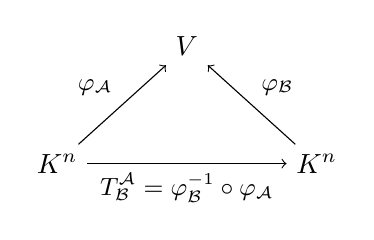
\begin{tikzpicture}
            \node (v) {$V$};
            \node [below left=of v] (k1) {$K^n$};
            \node [below right=of v] (k2) {$K^n$};

            \draw [->] (k1) -- (v) node [midway, above left] {\small $\varphi_{\mathcal{A}}$};
            \draw [->] (k2) -- (v) node [midway, above right] {\small $\varphi_{\mathcal{B}}$};
            \draw [->] (k1) -- (k2) node [midway, below] {\small $T^{\mathcal{A}}_{\mathcal{B}} = \varphi_{\mathcal{B}}^{-1} \circ \varphi_{\mathcal{A}}$};
        \end{tikzpicture}
    \end{center}


    Die Matrix $T^{\mathcal{A}}_{\mathcal{B}}$ heißt \emph{Transformationsmatrix des Basiswechsels von} $\mathcal{A}$ \emph{nach} $\mathcal{B}$

    Sei $v\in V$ beliebig, $K_{\mathcal{A}}(v) = \vektor{x_1 & \ldots & x_n}^T$ und $K_{\mathcal{B}}(v) = \vektor{y_1 & \ldots & y_n}^T$. Dann gilt:
    $$
        \vektor{y_1 \\ \vdots \\ y_n} = T^{\mathcal{A}}_{\mathcal{B}} \vektor{x_1 \\ \vdots \\ x_n}
    $$

    Sind die Koordinaten von $v$ beqüglich $\mathcal{A}$ bekannt, kann man mithilfe der Matrix $T^{\mathcal{A}}_{\mathcal{B}}$ die Koordinaten von $v$ bezüglich $\mathcal{B}$ berechnen.

    Seien $A$ und $B$ die Matrizen der Basisvektoren von $\mathcal{A}$ bzw. $\mathcal{B}$.
    Dann gilt:

    \begin{center}
        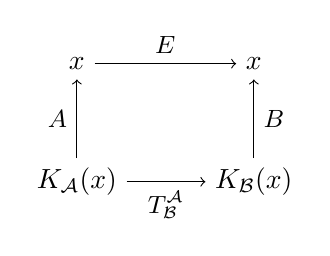
\begin{tikzpicture}
            \node (ka) {$K_{\mathcal{A}}(x)$};
            \node [right=of ka] (kb) {$K_{\mathcal{B}}(x)$};

            \node [above=of ka] (x1) {$x$};
            \node [above=of kb] (x2) {$x$};


            \draw [->] (x1) -- (x2) node [midway, above] {\small $E$};
            \draw [->] (ka) -- (x1) node [midway, left] {\small $A$};
            \draw [->] (kb) -- (x2) node [midway, right] {\small $B$};
            \draw [->] (ka) -- (kb) node [midway, below] {\small $T^{\mathcal{A}}_{\mathcal{B}}$};
        \end{tikzpicture}
    \end{center}

    Man erkennt:
    $$
        T^{\mathcal{A}}_{\mathcal{B}} = B^{-1}A
    $$
\end{defi}

\begin{example}{Transformationsmatrizen}
    $\mathcal{A}  = (e_1, e_2, e_3)$, $\mathcal{A}' = (a'_1, a'_2, a'_3)$ und $\mathcal{A}'' = (a''_1, a''_2, a''_3)$ bilden mit den kanonischen Einheitsvektoren $e_1, e_2, e_3$ sowie
    $$
        a'_1 = \vektor{1\\0\\0}, a'_2 = \vektor{1\\1\\0}, a'_3 = \vektor{1\\1\\1}
        \quad \text{bzw.} \quad
        a''_1 = \vektor{1\\-1\\0}, a''_2 = \vektor{-1\\0\\1}, a''_3 = \vektor{0\\1\\1}
    $$
    jeweils Basen des $\R^3$.

    Bestimmen Sie:
    \begin{enumerate}[a)]
        \item die Transformationsmatrizen $T^{\mathcal{A}'}_{\mathcal{A}}$ sowie $T^{\mathcal{A}}_{\mathcal{A}'}$.
        \item die Transformationsmatrizen $T^{\mathcal{A}''}_{\mathcal{A}}$ sowie $T^{\mathcal{A}}_{\mathcal{A}''}$.
        \item die Transformationsmatrizen $T^{\mathcal{A}'}_{\mathcal{A}''}$ sowie $T^{\mathcal{A}''}_{\mathcal{A}'}$.
        \item die Koordinaten des Vektors $\vektor{1 & 0 & 1}^T$ bzgl. der Basen $\mathcal{A}'$ und $\mathcal{A}''$.
    \end{enumerate}

    \exampleseparator

    \begin{enumerate}[a)]
        \item Berechnen von $\mathcal{A}'^{-1}$:
              $$
                  \begin{sysmatrix}{rrr|rrr}
                      1 & 1 & 1 & 1 & 0 & 0 \\
                      0 & 1 & 1 & 0 & 1 & 0 \\
                      0 & 0 & 1 & 0 & 0 & 1
                  \end{sysmatrix}
                  \sim
                  \begin{sysmatrix}{rrr|rrr}
                      1 & 1 & 0 & 1 & 0 & -1 \\
                      0 & 1 & 0 & 0 & 1 & -1 \\
                      0 & 0 & 1 & 0 & 0 & 1
                  \end{sysmatrix}
                  \sim
                  \begin{sysmatrix}{rrr|rrr}
                      1 & 0 & 0 & 1 & -1 & 0 \\
                      0 & 1 & 0 & 0 & 1 & -1 \\
                      0 & 0 & 1 & 0 & 0 & 1
                  \end{sysmatrix}
              $$

              Damit gilt:
              $$
                  T^{\mathcal{A}'}_{\mathcal{A}} = \mathcal{A}^{-1}\mathcal{A}' = \vektor{1 & 0 & 0 \\ 0 & 1 & 0 \\ 0 & 0 & 1} \vektor{1 & 1 & 1 \\ 0 & 1 & 1 \\ 0 & 0 & 1} = \vektor{1 & 1 & 1 \\ 0 & 1 & 1 \\ 0 & 0 & 1}
              $$
              und
              $$
                  T^{\mathcal{A}}_{\mathcal{A}'} = \mathcal{A}'^{-1}\mathcal{A} = \vektor{1 & -1 & 0 \\ 0 & 1 & -1 \\ 0 & 0 & 1} \vektor{1 & 0 & 0 \\ 0 & 1 & 0 \\ 0 & 0 & 1} = \vektor{1 & -1 & 0 \\ 0 & 1 & -1 \\ 0 & 0 & 1}.
              $$\qed
        \item Berechnen von $\mathcal{A}''^{-1}$:
              $$
                  \begin{sysmatrix}{rrr|rrr}
                      1 & -1 & 0 & 1 & 0 & 0 \\
                      -1 & 0 & 1 & 0 & 1 & 0 \\
                      0 & 1 & 1 & 0 & 0 & 1
                  \end{sysmatrix}
                  \sim
                  \ldots
                  \sim
                  \begin{sysmatrix}{rrr|rrr}
                      1 & 0 & 0 & \nicefrac{1}{2} & -\nicefrac{1}{2} & \nicefrac{1}{2} \\
                      0 & 1 & 0 & -\nicefrac{1}{2} & -\nicefrac{1}{2} & \nicefrac{1}{2}\\
                      0 & 0 & 1 & \nicefrac{1}{2} & \nicefrac{1}{2} & \nicefrac{1}{2}
                  \end{sysmatrix}
                  =
                  \frac{1}{2}\vektor{1 & -1 & 1 \\ -1 & -1 & 1 \\ 1 & 1 & 1}
              $$
              Damit gilt:
              $$
                  T^{\mathcal{A}''}_{\mathcal{A}} = \mathcal{A}^{-1}\mathcal{A}'' = \vektor{1 & 0 & 0 \\ 0 & 1 & 0 \\ 0 & 0 & 1} \vektor{1 & -1 & 0 \\ -1 & 0 & 1 \\ 0 & 1 & 1} = \vektor{1 & -1 & 0 \\ -1 & 0 & 1 \\ 0 & 1 & 1}
              $$
              und
              $$
                  T^{\mathcal{A}}_{\mathcal{A}''} = \mathcal{A}''^{-1}\mathcal{A} = \frac{1}{2}\vektor{1 & -1 & 1 \\ -1 & -1 & 1 \\ 1 & 1 & 1} \vektor{1 & 0 & 0 \\ 0 & 1 & 0 \\ 0 & 0 & 1} = \frac{1}{2}\vektor{1 & -1 & 1 \\ -1 & -1 & 1 \\ 1 & 1 & 1}.
              $$\qed
    \end{enumerate}

\end{example}

\begin{example}{Transformationsmatrizen (Fortsetzung)}
    \begin{enumerate}[a)]
        \setcounter{enumi}{2}
        \item Mit den bisherigen Ergebnissen gilt:
              $$
                  T^{\mathcal{A}'}_{\mathcal{A}''} = \mathcal{A}''^{-1}\mathcal{A}' = \frac{1}{2}\vektor{1 & -1 & 1 \\ -1 & -1 & 1 \\ 1 & 1 & 1} \vektor{1 & 1 & 1 \\ 0 & 1 & 1 \\ 0 & 0 & 1} = \frac{1}{2}\vektor{1 & 0 & 1 \\ -1 & -2 & -1 \\ 1 & 2 & 3}
              $$
              und
              $$
                  T^{\mathcal{A}''}_{\mathcal{A}'} = \mathcal{A}'^{-1}\mathcal{A}'' = \vektor{1 & -1 & 0 \\ 0 & 1 & -1 \\ 0 & 0 & 1} \vektor{1 & -1 & 0 \\ -1 & 0 & 1 \\ 0 & 1 & 1} = \vektor{2 & -1 & -1 \\ -1 & -1 & 0 \\ 0 & 1 & 1}.
              $$\qed
        \item Sei $x = \vektor{1 & 0 & 1}^T$.

              Dann gilt für $x$ bzgl. $\mathcal{A}'$:
              $$
                  x = K_{\mathcal{A}'}(x) = T^{\mathcal{A}}_{\mathcal{A}'} \cdot K_{\mathcal{A}}(x) = \vektor{1 & -1 & 0 \\ 0 & 1 & -1 \\ 0 & 0 & 1} \vektor{1 \\ 0 \\ 1} = \vektor{1 \\ -1 \\ 1},
              $$
              bzw. bzgl. $\mathcal{A}''$:
              $$
                  x = K_{\mathcal{A}''}(x) = T^{\mathcal{A}}_{\mathcal{A}''} \cdot K_{\mathcal{A}}(x) = \frac{1}{2}\vektor{1 & -1 & 1 \\ -1 & -1 & 1 \\ 1 & 1 & 1} \vektor{1 \\ 0 \\ 1} = \vektor{1 \\ 0 \\ 1}.
              $$\qed
    \end{enumerate}
\end{example}

\begin{defi}{Darstellungsmatrix mit Basistransformation}
    Seien $V$ und $W$ endlich erzeugt mit Basen $\mathcal{A}$ und $\mathcal{A}'$ bzw. $\mathcal{B}$ und $\mathcal{B}'$.
    Sei weiter $f : V \to W$ linear.
    Dann gilt:
    $$
        M^{\mathcal{A}'}_{\mathcal{\mathcal{B}'}}(f) = T^{\mathcal{B}}_{\mathcal{B}'} \cdot M^{\mathcal{A}}_{\mathcal{\mathcal{B}}}(f) \cdot T^{\mathcal{A}'}_{\mathcal{A}}
    $$

    Zur Visualisierung dient folgendes kommutative Diagramm:
    \begin{center}
        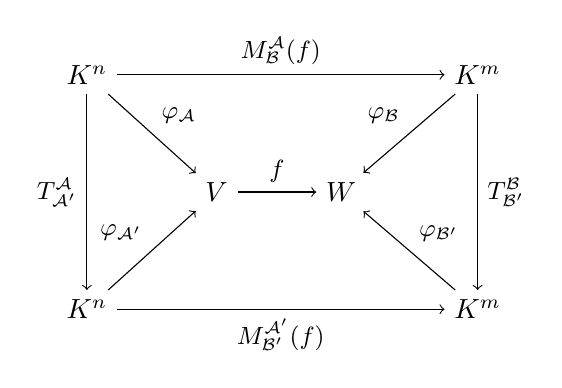
\begin{tikzpicture}
            \node (kn1) {$K^n$};
            \node [above right=of kn1] (v) {$V$};
            \node [above left=of v] (kn2) {$K^n$};
            \node [right=of v] (w) {$W$};
            \node [above right=of w] (km2) {$K^m$};
            \node [below right=of w] (km1) {$K^m$};

            \draw [->] (kn1) -- (v) node [midway, above left] {\small $\varphi_{\mathcal{A}'}$};
            \draw [->] (kn2) -- (v) node [midway, above right] {\small $\varphi_{\mathcal{A}}$};
            \draw [->] (km1) -- (w) node [midway, above right] {\small $\varphi_{\mathcal{B}'}$};
            \draw [->] (km2) -- (w) node [midway, above left] {\small $\varphi_{\mathcal{B}}$};

            \draw [->] (v) -- (w) node [midway, above] {\small $f$};

            \draw [->] (kn2) -- (km2) node [midway, above] {\small $M^{\mathcal{A}}_{\mathcal{B}} (f)$};
            \draw [->] (kn1) -- (km1) node [midway, below] {\small $M^{\mathcal{A}'}_{\mathcal{B}'} (f)$};

            \draw [->] (kn2) -- (kn1) node [midway, left] {\small $T^{\mathcal{A}}_{\mathcal{A}'}$};
            \draw [->] (km2) -- (km1) node [midway, right] {\small $T^{\mathcal{B}}_{\mathcal{B}'}$};
        \end{tikzpicture}
    \end{center}
\end{defi}

\section{Determinanten}

\begin{defi}{Elementarmatrix}
    Seien $1\leq i$, $j \leq n$ mit $i \neq j$ und $\lambda \in K \setminus \{0\}$ gegeben.
    Dann sei
    $$
        C1 := \vektor{1 & & & & \\ & \ddots & & & \\ & \lambda & \ddots & & \\ & & & \ddots & & \\ & & & & \ddots & \\ & & & & & 1} \in K^{n \times n}
    $$
    wobei der $(i, j)$-te Eintrag den Wert $\lambda$ annehmen soll und alle anderen Einträge außerhalb der Hauptdiagonalen $0$ sein sollen.

    Sei $C2$ die Matrix, die man aus der Einheitsmatrix gewinnt, indem man die $i$-te und $j$-te Spalte vertauscht, also
    $$
        C2 := \vektor{1 & & & & \\ & \ddots & & & \\ &  & 0 & &1 \\ & & & \ddots & & \\ & & 1 & & 0 & \\ & & & & & 1} \in K^{n \times n}
    $$

    Zuletzt definieren wir
    $$
        C3 := \vektor{1 & & & & \\ & \ddots & & & \\ &  & \lambda & & \\ & & & \ddots & & \\ & & & & \ddots & \\ & & & & & 1} \in K^{n \times n}
    $$

    Matrizen der Gestalt $C1$, $C2$ oder $C3$ nennt man \emph{Elementarmatrizen}.

    Es gilt:
    \begin{itemize}
        \item Die Multiplikation einer Matrix $A$ von links mit einer Elementarmatrix entspricht der Anwendung einer elementaren Zeilenoperation des Gauß-Verfahrens auf $A$.
              \subitem Notation: $Zi$ statt $Ci$
        \item Die Multiplikation einer Matrix $A$ von rechts mit einer Elementarmatrix entspricht der Anwendung einer elementaren Spaltenoperation auf $A$.
              \subitem Notation: $Si$ statt $Ci$
    \end{itemize}

    \begin{itemize}
        \item $C1$ entspricht dem Addieren von $\lambda$-mal Spalte bzw. Zeile $j$ auf Spalte bzw. Zeile $i$.
        \item $C2$ entspricht dem Tauschen von Spalte bzw. Zeile $i$ mit Spalte bzw. Zeile $j$.
        \item $C3$ entspricht dem Multiplizieren von Spalte bzw. Zeile $i$ mit $\lambda$.
    \end{itemize}
\end{defi}

\begin{example}{Elementarmatrizen}
    Sei
    $$
        A = \vektor{1 & 0 \\ -5 & 2}
    $$
    Bestimmen Sie Elementarmatrizen $M_1$ und $M_2$ mit $M_1M_2A = E$.

    \exampleseparator

    Es gilt:
    $$
        \begin{sysmatrix}{cc|cc}
            1 & 0 & 1 & 0 \\
            -5 & 2 & 0 & 1
        \end{sysmatrix}
        \sim
        \begin{sysmatrix}{cc|cc}
            1 & 0 & 1 & 0 \\
            0 & 2 & 5 & 1
        \end{sysmatrix}
        \sim
        \begin{sysmatrix}{cc|cc}
            1 & 0 & 1 & 0 \\
            0 & 1 & \frac{5}{2} & \frac{1}{2}
        \end{sysmatrix}
    $$
    Damit gilt:
    $$
        A^{-1} = \vektor{1 & 0 \\ \frac{5}{2} & \frac{1}{2}} =\footnote{Das wird aus dem Kontext ersichtlich: Für $A^{-1}$ wird zuerst fünfmal \Rnum{1} auf \Rnum{2} addiert und anschließend wird \Rnum{2} mit $\frac{1}{2}$ skaliert.} \vektor{1 & 0 \\ 0 & \frac{1}{2}} \cdot \vektor{1 & 0 \\ 5 & 1}
    $$
    und schlussendlich:
    $$
        A^{-1} \cdot A = \vektor{1 & 0 \\ 0 & \frac{1}{2}} \cdot \vektor{1 & 0 \\ 5 & 1} \cdot A = M_1 M_2  A
    $$\qed
\end{example}

\begin{defi}{Eigenschaften der Determinante}
    Für $A, B \in K^{n\times n}$ gilt:
    \begin{itemize}
        \item $S1$ und $Z1$ ändern die Determinante einer Matrix nicht. ($\det(C1) = 1$)
        \item $S2$ und $Z2$ kehren das Vorzeichen der Determinante um. ($\det(C2) = -1$)
        \item $S3$ und $Z3$ vervielfachen den Wert der Determinante um den Faktor $\lambda$. ($\det(C3) = \lambda$)
    \end{itemize}

    \begin{itemize}
        \item $\det(A) = \det(A^T)$
        \item Besitzt $A$ zwei gleiche Spalten bzw. Zeilen, so gilt $\det(A) = 0$.
        \item $A$ invertierbar $\iff \det(A) \neq 0$
        \item $\det(AB) = \det(A)\det(B)$
        \item $A$ invertierbar $\implies \det(A^{-1}) = (\det(A))^{-1}$
    \end{itemize}
\end{defi}

\subsection{Verfahren zur Berechnung der Determinante}

\begin{defi}{Laplacescher Entwicklungssatz}
    Für $A \in K^{n\times n}$ bezeichne $A_{ij}$ die Matrix in $K^{(n-1)\times (n-1)}$, die durch Streichen der $i$-ten Zeile und der $j$-ten Spalte aus $A$ hervorgeht.

    Es sei $A = (a_{ij}) \in K^{n\times n}$ und $j$ mit $1 \leq j \leq n$.
    Dann gilt:
    $$
        \det(A) = \sum^n_{i=1} (-1)^{i+j} a_{ij}\det(A_{ij})
    $$
    Man spricht von der \emph{Entwicklung der Determinante nach der j-ten Spalte}.
    Ebenso ist eine \emph{Entwicklung der Determinante nach der i-ten Zeile} möglich:
    $$
        \det(A) = \sum^n_{j=1} (-1)^{i+j} a_{ij}\det(A_{ij})
    $$
\end{defi}

\begin{defi}{Determinante mit Gauß-Algorithmus}
    Zur Berechnung mit dem Gauß-Algorithmus bringt man die gegebene Matrix $A$ mittels äquivalenter Zeilen- oder Spaltenumformungen $Z1$-$Z3$ bzw. $S1$-$S3$ auf Stufenform $B$ und errechnet dann nach Folgerung $\det(A)$ leicht als Produkt der Hauptdiagonalelelemente von $B$, multipliziert mit den Determinanten der genutzten Elementarmatrizen.
\end{defi}

\begin{example}{Determinante mit Gauß-Algorithmus}
    Berechnen Sie die Determinante von $A = \vektor{4 & 5 & 6 \\ 2 & -2 & -1 \\ 0 & 1 & -3}$ mit Hilfe des Gauß-Algorithmus.

    \exampleseparator

    $$
        \vektor{4 & 5 & 6 \\ 2 & -2 & -1 \\ 0 & 1 & -3}
        \underset{}{\xrightarrow{\text{\Rnum{2}: \Rnum{2} + 2 \Rnum{3}}}}
        \vektor{4 & 5 & 6 \\ 2 & 0 & -7 \\ 0 & 1 & -3}
        \underset{}{\xrightarrow{\text{\Rnum{1}: \Rnum{1} - 5 \Rnum{3}}}}
        \vektor{4 & 0 & 21 \\ 2 & 0 & -7 \\ 0 & 1 & -3}
        \underset{}{\xrightarrow{\text{\Rnum{1}: \Rnum{1} - 2 \Rnum{2}}}}
        \vektor{0 & 0 & 35 \\ 2 & 0 & -7 \\ 0 & 1 & -3}
    $$
    $$
        \vektor{0 & 0 & 35 \\ 2 & 0 & -7 \\ 0 & 1 & -3}
        \underset{\nicefrac{1}{35} \cdot \det(A)}{\xrightarrow{\text{\Rnum{1}: \Rnum{1} - 2 \Rnum{2}}}}
        \vektor{0 & 0 & 1 \\ 2 & 0 & -7 \\ 0 & 1 & -3}
        \underset{}{\xrightarrow{\text{(\Rnum{2}: \Rnum{2} + 7 \Rnum{1})} \ \circ \ \text{(\Rnum{3}: \Rnum{3} + 3 \Rnum{1})}}}
        \vektor{0 & 0 & 1 \\ 2 & 0 & 0 \\ 0 & 1 & 0}
    $$
    $$
        \vektor{0 & 0 & 1 \\ 2 & 0 & 0 \\ 0 & 1 & 0}
        \underset{(-1)\cdot(-1)\cdot \det A}{\xrightarrow{\text{(\Rnum{1}$\,\leftrightarrow\,$\Rnum{3})} \ \circ \ \text{(\Rnum{1}$\,\leftrightarrow\,$\Rnum{2})}}}
        \vektor{2 & 0 & 0 \\ 0 & 1 & 0 \\ 0 & 0 & 1}
    $$
    Damit gilt:
    $$
        \det A = (-1) \cdot (-1) \cdot 35 \cdot \dvektor{2 & 0 & 0 \\ 0 & 1 & 0 \\ 0 & 0 & 1} = 35 \cdot 2 = 70
    $$\qed
\end{example}

\begin{bonus}{Tipps zur Determinantenberechnung}
    \begin{enumerate}
        \item Für $(2\times 2)$- und $(3\times 3)$-Matrizen empfiehlt sich die Sarrus-Regel.\footnote{Siehe Lineare Algebra 1}
        \item Die Laplace-Entwicklung ist dann vorzuziehen, wenn in einer Spalte oder Zeile nur wenige Nicht-Null-Einträge vorhanden sind, weil bei einer Entwicklung nach dieser Zeile bzw. Spalte die meisten Summanden erst gar nicht berechnet werden müssen.
        \item Es können zur Berechnung der Determinanten mehrere Verfahren kombiniert werden, z.B. $(4\times 4)$-Matrizen zuerst nach Laplace entwickeln und die dann entstehenden Determinanten von $(3\times 3)$-Matrizen direkt mit der Sarrus-Regel berechnen.
    \end{enumerate}
\end{bonus}

\begin{bonus}{Inverse einer $(2\times 2)$-Matrix}
    Sei $A$ definiert als $A = \vektor{a & b \\ c & d}$. Dann gilt:
    $$
        A^{-1} = \frac{1}{\det(A)} \vektor{d & -b \\ -c & a} = \frac{1}{ad - bc} \vektor{d & -b \\ -c & a}
    $$
\end{bonus}

\section{Lineare Gleichungssysteme}

\subsection{Lösbarkeit eines linearen Gleichungssystems}

\begin{defi}{Lineares Gleichungssystem}
    Seien $A = (a_{ij}) \in K^{m\times n}$ und $b = \vektor{b_1 & \ldots & b_m}^T$.
    Dann heißt
    $$
        \begin{aligned}
             & a_{11}x_1 &  & + \ \ldots \ + &  & a_{1n}x_n &  & = &  & b_1 \\
             & \ldots                                                       \\
             & a_{m1}x_1 &  & + \ \ldots \ + &  & a_{mn}x_n &  & = &  & b_m
        \end{aligned}
    $$
    \emph{lineares Gleichungssystem} bzgl. $(x_1, \ldots, x_n)$ mit Koeffizienten $a_{ij}$ in $K$.
    Hierbei sind $x_1, \ldots, x_n$ die \emph{Unbekannten} des Systems.

    Für $b = 0_{m1}$ nennt man das lineare Gleichungssystem \emph{homogen}, sonst \emph{inhomogen}.

    Jedes lineare Gleichungssystem kann in der Form $Ax = b$ geschrieben werden.
\end{defi}

\begin{defi}{Lösungsmenge}
    Die \emph{Lösungsmenge} $L(A, b)$ des zu $(A, b)$ gehörigen Gleichungssystems ist festgelegt durch
    $$
        L(A, b) := \{x \in K^n \mid Ax = b\}
    $$
\end{defi}

\begin{defi}{Spaltenrang}
    Die lineare Abbildung $L_A : K^n \to K^m$ sei gegeben durch $L_A(x) := Ax$. Dann sei $\rg(A) := \rg(L_A)$.
    Der \emph{Spaltenrang} $\rg_S(A)$ sei die maximale Anzahl linear unabhängiger Spaltenvektoren von $A$.

    Es gilt $\rg(A) = \rg_S(A)$.
\end{defi}

\begin{defi}{Zeilenrang}
    Für $A \in K^{m\times n}$ sei die maximale Anzahl linear unabhängiger Zeilenvektoren von $A$ der \emph{Zeilenrang} $\rg_Z(A)$ von $A$.

    Es gilt:
    $$
        \rg(A) = \rg_S(A) = \rg_Z(A)
    $$
\end{defi}

\begin{defi}{Lösbarkeit von linearen Gleichungssystemen}
    Das lineare Gleichungssystem $Ax = b$ ist genau dann lösbar, wenn gilt:
    $$
        \rg(a_1, \ldots, a_n) = \rg(a_1, \ldots, a_n, b)
    $$
    Kürzer schreibt man $\rg(A) = \rg(A, b)$.

    $Ax = b$ ist also genau dann eindeutig lösbar, falls $\ker(A) = \{0\} \iff \rg(A) = \rg(A, b) = n$.
\end{defi}

\begin{bonus}{Äquivalente Bedingungen für eindeutige Lösbarkeit}
    Sei $K \in \{\R, \C\}$.
    Für $A \in K^{n\times n}$ und die dadurch gegebene lineare Abbildung $L_A$ sind folgende Bedingungen äquivalent:
    \begin{enumerate}
        \item $A$ ist invertierbar.
        \item $Ax = 0$ hat nur die triviale Lösung $x=0$.
        \item Durch Zeilen- und Spaltenumformungen kann $A$ auf die Einheitsmatrix transformiert werden.
        \item $A$ ist darstellbar als Produkt von Elementarmatrizen.
        \item $Ax = b$ besitzt für jedes $b \in K^n$ mindestens eine Lösung.
        \item $Ax = b$ hat genau eine Lösung für jedes $b \in K^n$.
        \item $\det(A) \neq 0$
        \item $\im(A) = K^n$
        \item $L_A$ ist bijektiv.
        \item Die Spaltenvektoren von $A$ sind linear unabhängig.
        \item Die Zeilenvektoren von $A$ sind linear unabhängig.
        \item Die Spaltenvektoren von $A$ bilden eine Basis von $K^n$.
        \item Die Zeilenvektoren von $A$ bilden eine Basis von $K^n$.
        \item $\rg(A)=n$
        \item $\ker(L_A) = \{0\}$
        \item $(\ker(L_A))^\perp = K^n$
        \item Das orthogonale Komplement des von den Zeilen von $A$ aufgespannten Raums ist $\{0\}$.
        \item $A^TA$ ist invertierbar.
    \end{enumerate}
\end{bonus}

\begin{defi}{Allgemeine Lösung eines linearen Gleichungssystems}
    Sei $x_s \in K^n$ eine (spezielle) Lösung von $Ax = b$.
    Dann gilt:
    $$
        L(A, b) = x_s + \ker(A) = \{x_s + x \mid x \in \ker(A)\}
    $$
    bzw., wenn $(v_1, \ldots, v_r)$ eine Basis von $\ker(A)$ ist:
    $$
        L(A, b) = \{x + \lambda_1 v_1 + \ldots + \lambda_rv_r \mid \lambda_i \in K\}
    $$
\end{defi}

\begin{example}{Allgemeine Lösung eines linearen Gleichungssystems}
    Finden Sie die Lösung des linearen Gleichungssystems
    $$
        \vektor{-1 & 1 & 0 \\ 0 & 1 & 1}x = \vektor{0 \\ 2}
    $$
    mit Hilfe folgender Schritte:
    \begin{enumerate}[a)]
        \item Bestimmen Sie den Kern der Abbildungsmatrix.
        \item Erraten Sie eine spezielle Lösung.
        \item Bestimmen Sie die allgemeine Lösung.
    \end{enumerate}

    \exampleseparator

    \begin{enumerate}[a)]
        \item $$
                  \begin{sysmatrix}{rrr|r}
                      -1 & 1 & 0 & 0 \\
                      0 & 1 & 1 & 0
                  \end{sysmatrix}
                  \quad \implies \quad
                  \ker \vektor{-1 & 1 & 0 \\ 0 & 1 & 1} = \scalarprod{\vektor{1 \\ 1 \\ -1}}
              $$\qed
        \item $$
                  x = \vektor{0\\0\\2} \quad \implies \quad \vektor{-1 & 1 & 0 \\ 0 & 1 & 1}\cdot \vektor{0\\0\\2} = \vektor{0 \\ 2}
              $$\qed
        \item Es gilt:
              $$
                  L \left({\vektor{-1 & 1 & 0 \\ 0 & 1 & 1}, \vektor{0 \\ 2}} \right) = \vektor{0\\0\\2} + \ker\vektor{-1 & 1 & 0 \\ 0 & 1 & 1} = \vektor{0\\0\\2} + \lambda \cdot \vektor{1 \\ 1 \\ -1}, \quad \lambda \in \R
              $$\qed
    \end{enumerate}
\end{example}

\begin{defi}{Cramersche Regel}
    Es seien $A = \vektor{a_1 & \ldots & a_n} \in K^{n\times n}$ und $x, b \in K^n$ sowie $Ax=b$ ein lineares Gleichungssystem, und es gelte $\det(A) \neq 0$.
    Seien
    $$
        A_i := \vektor{a_1 & \ldots & a_{i-1} & b & a_{i+1} & \ldots & a_n}, 1 \leq i \leq n
    $$
    Dann gilt:
    $$
        x_i = \frac{\det(A_i)}{\det(A)}
    $$
\end{defi}

\begin{example}{Cramersche Regel}
    In der Elektrotechnik ergeben sich eine Widerstandsmatrix $R$ und ein Quellspannungsvektor $U$:
    $$
        R = \vektor{1 & 3 & 0 \\ 1 & 4 & 1 \\ 2 & 1 & 1}, \quad U = \vektor{5 \\ 9 \\ 8}.
    $$
    Gesucht ist der Stromvektor $I$, der sich durch Lösen des linearen Gleichungssystems
    $$
        R \cdot I = U
    $$
    ergibt.
    Bestimmen Sie die Lösung mithilfe der Cramerschen Regel.

    \exampleseparator

    Es gilt:
    $$
        \vektor{1 & 3 & 0 \\ 1 & 4 & 1 \\ 2 & 1 & 1}  \vektor{i_1 \\ i_2 \\ i_3} = \vektor{5 \\ 9 \\ 8}
    $$

    Nach der Cramerschen Regel gilt:\footnote{$\abs{R} = -1 \cdot (1-6) + 1 \cdot (4-3) = 6$}
    $$
        i_1 = \frac{\dvektor{5 & 3 & 0 \\ 9 & 4 & 1 \\ 8 & 1 & 1}}{\abs{R}} = \frac{-1 \cdot (5-24) + 1 \cdot (20-27)}{6} = \frac{12}{6} = 2
    $$
    $$
        i_2 = \frac{\dvektor{1 & 5 & 0 \\ 1 & 9 & 1 \\ 2 & 8 & 1}}{\abs{R}} = \frac{-1 \cdot (8-10) + 1 \cdot (9-5)}{6} = \frac{6}{6} = 1
    $$
    $$
        i_3 = \frac{\dvektor{1 & 3 & 5 \\ 1 & 4 & 9 \\ 2 & 1 & 8}}{\abs{R}} = \frac{32+54+5-40-9-24}{6} = \frac{18}{6} = 3
    $$

    Damit ist der Stromvektor $I$ gegeben mit $I = \vektor{2 & 1 & 3}^T$.\qed
\end{example}

\subsection{Über- und unterbestimmte lineare Gleichungssysteme}

\begin{defi}{Normalgleichung}
    Sei $p_A(b)$ die Projektion eines Vektors $b \in \R^m$ auf den von den Vektoren $A = \vektor{a_1 & \ldots & a_n} \in \R^{m\times n}$ aufgespannten Unterraum $U$, also das Bild von $A$.

    Damit existiert ein $x \in \R^n$ mit
    $$
        p_A(b) = \sum^n_{k=1} x_ka_k = Ax
    $$
    Dann gilt
    $$
        b - p_A(b) \iff \ldots \iff A^TAx = A^Tb
    $$

    Die Gleichungen $A^TAx = A^Tb$ heißen \emph{Normalgleichungen}.

    Die Normalgleichungen sind für jede relle Matrix $A \in \R^{m\times n}$ lösbar.

\end{defi}

\begin{defi}{Verallgemeinerte Inverse}
    Gegeben ist ein lineares Gleichungssystem $Ax=b$ mit $A \in \R^{m\times n}$, $x \in \R^n$, $b \in \R^m$.

    Im Fall $\rg(A) = n$ (voller Spaltenrang) existiert mit
    $$
        x = (A^TA)^{-1}A^Tb
    $$
    eine eindeutige Lösung.
    In diesem Fall heißt $(A^TA)^{-1}A^T$ \emph{verallgemeinerte Inverse} von $A$.

    Im Fall $\rg(A) = m$ (voller Zeilenrang) existiert mit
    $$
        x = A^T(AA^T)^{-1}b
    $$
    eine eindeutige Lösung.
    In diesem Fall heißt $A^T(AA^T)^{-1}$ \emph{verallgemeinerte Inverse} von $A$.
\end{defi}

\begin{algo}{Lösen von überbestimmten Gleichungssystemen (Methode der kleinsten Quadrate)}
    Gegeben ist das \emph{überbestimmte} Gleichungssystem
    $$
        Ax = b, \quad A \in \R^{m\times n}, \, b\in \R^m, \, m \geq n
    $$
    Im Fall $\rg(A) = n$ (voller Spaltenrang) gilt mithilfe der verallgemeinerten Inverse für
    $$
        x_s = (A^TA)^{-1}A^Tb
    $$
    dass
    $$
        \norm{b-Ax_s} = \min_{z\in\R^n} \norm{b-Az}
    $$

    Der Vektor $x_s$ heißt \emph{Näherungslösung nach der Methode der kleinsten Quadrate}.
\end{algo}

\begin{example}{Methode der kleinsten Quadrate}
    Eine Messreihe ergibt zu den Zeiten $t = 1,2,3,4,5$ in Sekunden folgende Temperaturwerte:

    \begin{center}
        \begin{tabular}{l | CCCCC}
            $t$ Sekunden        & 1   & 2   & 3    & 4    & 5    \\
            \hline
            $y(t)\si{\celsius}$ & 0.9 & 5.8 & 11.4 & 12.1 & 12.9 \\
        \end{tabular}
    \end{center}

    Stellen Sie das überbestimmte Gleichungssystem für die unbekannten Parameter $a$ und $b$ auf und bestimmen Sie diese nach der Methode der kleinsten Quadrate, wenn folgende Beziehung zwischen $y$ und $t$ gilt:
    $$
        y(t) = a \cdot t + b \cdot \sin\left( -t \cdot \frac{\pi}{2} \right)
    $$
    \exampleseparator

    \begin{center}
        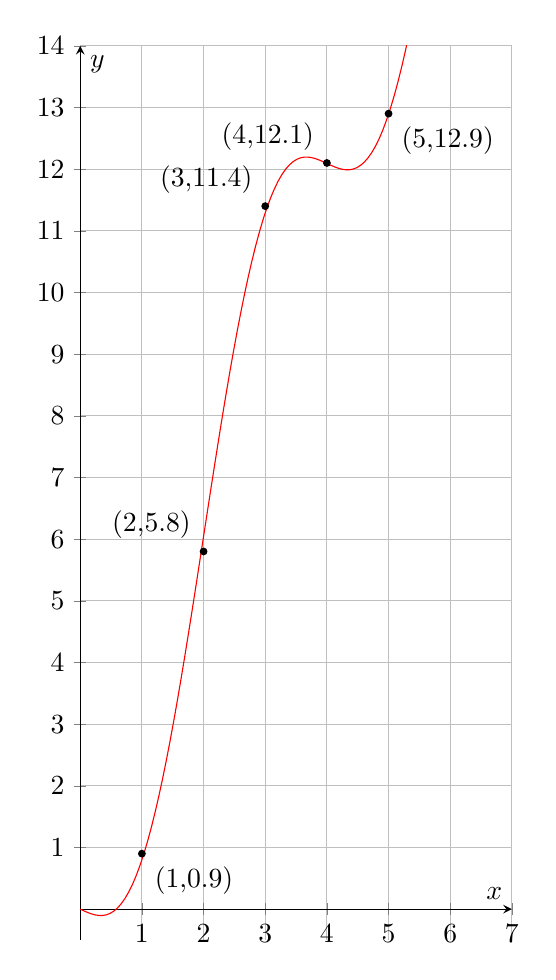
\begin{tikzpicture}[scale=1]
            \begin{axis}[
                    %view={45}{15},
                    width=15cm,
                    unit vector ratio*=1 1,
                    axis lines = middle,
                    grid=major,
                    ymin=-.5,
                    ymax=14,
                    xmin=0,
                    xmax=7,
                    %zmin=-1,
                    %zmax=10,
                    xlabel = $x$,
                    ylabel = $y$,
                    %zlabel = $z$,
                    %xtick style={draw=none},
                    %ytick style={draw=none},
                    %ztick style={draw=none},
                    xtick distance={1},
                    ytick distance={1},
                    %ztick distance={1},
                    %xticklabels=\empty,
                    %yticklabels=\empty,
                    %zticklabels=\empty,
                    disabledatascaling,
                ]

                \addplot[domain=0:6, samples=100, color=red]{3.02308 * x - 2.22308 * sin(deg(x * pi/2))};

                \node[label={315:{(1,0.9)}},circle,fill,inner sep=1pt] at (axis cs:1,0.9) {};
                \node[label={135:{(2,5.8)}},circle,fill,inner sep=1pt] at (axis cs:2,5.8) {};
                \node[label={135:{(3,11.4)}},circle,fill,inner sep=1pt] at (axis cs:3,11.4) {};
                \node[label={135:{(4,12.1)}},circle,fill,inner sep=1pt] at (axis cs:4,12.1) {};
                \node[label={315:{(5,12.9)}},circle,fill,inner sep=1pt] at (axis cs:5,12.9) {};
            \end{axis}
        \end{tikzpicture}
    \end{center}
\end{example}

\begin{example}{Methode der kleinsten Quadrate (Fortsetzung)}
    Mit den gegebenen Daten erhalten wir folgendes LGS:
    $$
        Ax = b \quad \iff \quad \vektor{1 & -\sin \frac{\pi}{2} \\ 2 & -\sin \pi \\ 3 & -\sin \frac{3\pi}{2} \\ 4 & -\sin 2 \pi \\ 5 & -\sin \frac{5\pi}{2}}\vektor{a \\ b} = \vektor{0.9 \\ 5.8 \\ 11.4 \\ 12.1 \\ 12.9} \quad \iff \quad \vektor{1 & -1 \\ 2 & 0 \\ 3 & 1 \\ 4 & 0 \\ 5 & -1}\vektor{a \\ b} = \vektor{0.9 \\ 5.8 \\ 11.4 \\ 12.1 \\ 12.9}
    $$
    mit
    $$
        \rg(A) = 2 = n \quad \implies \quad A^TAx = A^Tb \quad \iff \quad x = \left(A^T A\right)^{-1} A^T b
    $$
    Dann gilt nach der Methode der kleinsten Quadrate:
    $$
        \begin{aligned}
            x_s \quad = \quad & \left(A^T A\right)^{-1} A^T b                     \\
            = \quad           & \left(\vektor{1               & 2  & 3  & 4  & 5  \\ -1 & 0 & 1 & 0 & -1} \vektor{1 & -1 \\ 2 & 0 \\ 3 & 1 \\ 4 & 0 \\ 5 & -1}\right)^{-1} \vektor{1 & 2 & 3 & 4 & 5 \\ -1 & 0 & 1 & 0 & -1} \vektor{0.9 \\ 5.8 \\ 11.4 \\ 12.1 \\ 12.9} \\
            = \quad           & \vektor{55                    & -3                \\ -3 & 3}^{-1} \vektor{1 & 2 & 3 & 4 & 5 \\ -1 & 0 & 1 & 0 & -1} \vektor{0.9 \\ 5.8 \\ 11.4 \\ 12.1 \\ 12.9} \\
            = \quad           & \frac{1}{156}\vektor{3        & 3                 \\ 3 & 55} \vektor{1 & 2 & 3 & 4 & 5 \\ -1 & 0 & 1 & 0 & -1} \vektor{0.9 \\ 5.8 \\ 11.4 \\ 12.1 \\ 12.9} \\
            = \quad           & \frac{1}{156}\vektor{0        & 6  & 12 & 12 & 12 \\ -52 & 6 & 64 & 12 & -40} \vektor{0.9 \\ 5.8 \\ 11.4 \\ 12.1 \\ 12.9} \\
            = \quad           & \frac{1}{156}\vektor{471.6                        \\ 346.8} = \vektor{3.02308 \\ 2.22308} = \vektor{a \\ b}
        \end{aligned}
    $$

    Damit gilt insgesamt:
    $$
        y(t) = a \cdot t + b \cdot \sin\left( -t \cdot \frac{\pi}{2} \right) = 3.02308 \cdot t + 2.22308 \cdot \sin\left( -t \cdot \frac{\pi}{2} \right)
    $$\qed
\end{example}


\begin{algo}{Lösen von unterbestimmten Gleichungssystemen}
    Gegeben ist das \emph{unterbestimmte} Gleichungssystem
    $$
        Ax = b, \quad A \in \R^{m\times n}, \, b\in \R^m, \, m \leq n
    $$
    Im Fall $\rg(A) = m$ (voller Zeilenrang) gilt mithilfe der verallgemeinerten Inverse für
    $$
        x_s = A^T(AA^T)^{-1}b
    $$
    dass
    $$
        \norm{x_s} = \min_{Ax=b} \norm{x} \quad \land \quad x_s \perp \ker(A)
    $$

    Der Vektor $x_s$ ist eine \emph{eindeutige Lösung mit minimaler Norm}.
\end{algo}

\begin{example}{Lösen von unterbestimmten Gleichungssystemen}
    Die Punkte $A(6;0;0)$, $B(2;1;3)$ und $C(-2;-2;2)$ liegen in einer Ebene $E$.
    \begin{enumerate}[a)]
        \item Stellen Sie die Hessesche Normalform der Ebene auf.
              Wie groß ist der Abstand der Ebene zum Ursprung?
        \item Welcher Punkt in der Ebene hat den kleinsten Abstand zum Ursprung?
              Stellen Sie dazu das zugehörige unterbestimmte LGS auf und finden Sie die Lösung mit Hilfe der verallgemeinerten Inverse.
    \end{enumerate}

    \exampleseparator

    \begin{enumerate}[a)]
        \item Wir wählen uns $\vec{a}$ (Ortsvektor von $A$) als Stützvektor und die Vektoren $v = \vec{b} - \vec{a}$ und $w = \vec{c} - \vec{a}$ als Richtungsvektoren der Ebene.
              Dann gilt:
              $$
                  v = \vektor{2\\1\\3} - \vektor{6\\0\\0} = \vektor{-4\\1\\3}, \qquad w = \vektor{-2\\-2\\2} - \vektor{6\\0\\0} = \vektor{-8\\-2\\2}
              $$
              $$
                  n = \frac{v \times w}{\abs{v \times w}} = \frac{1}{\abs{v \times w}} \vektor{8 \\ -16 \\ 16} = \frac{1}{24} \vektor{8 \\ -16 \\ 16} = \vektor{\nicefrac{1}{3} \\ -\nicefrac{2}{3} \\ \nicefrac{2}{3}}
              $$

              Mit $n$ als (normierten) Normalenvektor erhalten wir dann die Hessesche Normalform der Ebene mit
              $$
                  E: \scalarprod{x,n} = \scalarprod{\vec{a}, n} \quad \iff \quad \frac{1}{3} \cdot x - \frac{2}{3} \cdot y + \frac{2}{3} \cdot z = 2
              $$

              Setzen wir den Nullpunkt in die Ebene ein, erhalten wir den Abstand mit $d = 2$.\qed
        \item Mit der Ebenengleichung
              $$
                  E: \frac{1}{3} \cdot x - \frac{2}{3} \cdot y + \frac{2}{3} \cdot z = 2
              $$
              können wir folgendes unterbestimmte LGS aufstellen:
              $$
                  Ax = b \quad \iff \quad \vektor{\nicefrac{1}{3} & -\nicefrac{2}{3} & \nicefrac{2}{3}} \vektor{x \\ y \\ z} = \vektor{2}
              $$
              mit
              $$
                  \rg(A) = 1 = m \quad \implies \quad x = A^T \left(AA^T\right)^{-1}b
              $$

              Dann gilt:
              $$
                  \begin{aligned}
                      x_s \quad = \quad & A^T \left(AA^T\right)^{-1}b \\
                      = \quad           & \vektor{\nicefrac{1}{3}     \\ -\nicefrac{2}{3} \\ \nicefrac{2}{3}} \left( \vektor{\nicefrac{1}{3} & -\nicefrac{2}{3} & \nicefrac{2}{3}} \vektor{\nicefrac{1}{3} \\ -\nicefrac{2}{3} \\ \nicefrac{2}{3}} \right)^{-1} \cdot 2 \\
                      = \quad           & \vektor{\nicefrac{2}{3}     \\ -\nicefrac{4}{3} \\ \nicefrac{4}{3}} = \vektor{x\\y\\z}
                  \end{aligned}
              $$
              Damit ist dann $\vektor{\nicefrac{2}{3} & -\nicefrac{4}{3} & \nicefrac{4}{3}}^T$ der gesuchte Punkt in der Ebene mit dem geringsten Abstand.\qed
    \end{enumerate}
\end{example}
\section{Geometrie linearer Abbildungen}

\subsection{Orthogonale Abbildungen und Matrizen}

\begin{defi}{Isometrie}
    Eine \emph{Isometrie} ist eine lineare Abbildung, die zwei metrische Räume aufeinander abbildet und dabei die euklidische Länge eines Vektors erhält.

    Man spricht auch von einer abstandserhaltenden Abbildung.

    Sei $f : \R^n \to \R^n$ beliebig. Dann sind äquivalent:
    \begin{enumerate}
        \item $\forall x, y \in \R^n : \scalarprod{f(x), f(y)} = \scalarprod{x, y}$
        \item $f$ ist eine winkelerhaltende Isometrie.
    \end{enumerate}
\end{defi}

\begin{defi}{Orthogonalmatrix}
    Eine Matrix $A\in \R^{n\times n}$ heißt \emph{orthogonal}, wenn ihre Spaltenvektoren eine Orthonormalbasis bilden.

    Die Menge aller orthogonalen Matrizen in $\R^{n\times n}$ heiße $O(n)$.

    Es gilt:
    \begin{itemize}
        \item $A \in O(n) \implies \abs{\det(A)} = 1$
    \end{itemize}

    Es sind äquivalent:
    \begin{enumerate}
        \item $A \in O(n)$
        \item $A$ ist invertierbar, und es gilt $A^{-1} = A^T$
        \item $A^T \in O(n)$
    \end{enumerate}
\end{defi}

\begin{example}{Orthogonalmatrix}
    Zeigen Sie, dass die Matrix
    $$
        Q = \vektor{
            \cos \beta & -\sin\beta & 0 \\
            \cos \alpha \sin\beta & \cos\alpha \cos\beta & -\sin\alpha \\
            \sin\alpha \sin\beta & \sin\alpha \cos\beta & \cos\alpha
        }
    $$
    eine Orthogonalmatrix ist und bestimmen Sie ihre Inverse.

    \exampleseparator

    Genau dann, wenn $Q$ eine Orthogonalmatrix ist, ist $QQ^T = I$ und damit auch $Q^T = Q^{-1}$:
    $$
        \begin{aligned}
            QQ^T = \quad        &
            \vektor{ \cos \beta & -\sin\beta                        & 0                        \\ \cos \alpha \sin\beta & \cos\alpha \cos\beta & -\sin\alpha \\ \sin\alpha \sin\beta & \sin\alpha \cos\beta & \cos\alpha }
            \vektor{ \cos\beta  & \cos\alpha \sin\beta              & \sin\alpha \sin\beta     \\ -\sin\beta & \cos\alpha \cos\beta & \sin\alpha \cos\beta \\ 0 & -\sin\alpha & \cos\alpha} \\
            = \quad             & \vektor{\cos^2\beta + \sin^2\beta & 0                    & 0 \\ 0 & \cos^2\alpha \left( \sin^2\beta + \cos^2\beta \right) + \sin^2\alpha & 0  \\ 0 & 0 & \sin^2\alpha \left( \sin^2\beta + \cos^2\beta \right) + \cos^2\alpha} \\
            = \quad             & \vektor{\cos^2\beta + \sin^2\beta & 0                    & 0 \\ 0 & \cos^2\alpha  + \sin^2\alpha & 0  \\ 0 & 0 & \sin^2\alpha + \cos^2\alpha} \\
            = \quad             & \vektor{1                         & 0                    & 0 \\ 0 & 1 & 0  \\ 0 & 0 & 1}
        \end{aligned}
    $$

    Damit ist $Q$ eine Orthogonalmatrix und $Q^T$ die Inverse von $Q$.\qed
\end{example}

\begin{algo}{QR-Zerlegung}
    Sei $A = \vektor{a_1 & \ldots & a_n} \in \R^{m\times n}$ und $\rg(A) = n$.
    Dann gibt es eine in den Spalten orthogonale Matrix $Q \in \R^{m\times n}$ und eine obere Dreiecksmatrix $R \in \R^{n\times n}$ mit $A = QR$.
    Hierbei können die Spalten von $Q$ mithilfe des Verfahrens von Gram-Schmidt aus den Spalten von $A$ erzeugt werden, und es gilt $\rg(R) = n$.

    Mit $Q = \vektor{q_1 & \ldots & q_n}$ und $R = (\varrho_{ij})$ ergibt sich $R$ durch Lösen der $n$ linearen Gleichungen
    $$
        \vektor{a_1 & \ldots & a_n} = \vektor{q_1 & \ldots & q_n} \vektor{ \varrho_{11} & \varrho_{12} & \ldots & \varrho_{1n} \\ & \varrho_{22} & \ldots & \varrho_{2n} \\ & & \ddots & \vdots \\ & & & \varrho_{nn}}
    $$
    Hierbei kann bei $n > 1$ über die per Gram-Schmidt generierten Zwischenrechnungen durch Koeffizientenvergleich gelöst werden.
\end{algo}

\begin{example}{QR-Zerlegung}
    Wie lautet die QR-Zerlegung von
    $$
        A = \vektor{3 & 1 \\ 4 & 5}?
    $$
    Lösen Sie anschließend mit dieser Zerlegung das lineare Gleichungssystem $Ax = b$ mit $b = \vektor{2 & 3}^T$.

    \exampleseparator

    Wir wenden das Gram-Schmidt-Verfahren auf die Spaltenvektoren an:\footnote{Wir sehen, dass die Vektoren orthogonal sind.}
    $$
        \begin{aligned}
            v_1 \quad = \quad & \vektor{3                                                        \\4} \\
            w_1 \quad = \quad & \frac{v_1}{\norm{v_1}} = \frac{1}{5}\vektor{3                    \\4} = \vektor{\nicefrac{3}{5}\\\nicefrac{4}{5}} \\
            v_2 \quad = \quad & \vektor{1                                                        \\5} \\
            r_2 \quad = \quad & v_2 - \scalarprod{v_2, w_1}w_1                                   \\
            = \quad           & \vektor{1                                                        \\ 5} - \left( \frac{1}{5} \right)^2\scalarprod{\vektor{1 \\ 5}, \vektor{3 \\ 4}}\vektor{3 \\ 4} =  \vektor{-\nicefrac{44}{25}                      \\ \nicefrac{33}{25}}\\
            w_2 \quad = \quad & \frac{r_2}{\norm{r_2}} = \frac{5}{11} \vektor{-\nicefrac{44}{25} \\ \nicefrac{33}{25}} = \vektor{-\nicefrac{4}{5} \\ \nicefrac{3}{5}}
        \end{aligned}
    $$

    Damit erhalten wir $Q$ mit
    $$
        Q = \vektor{w_1 & w_2} =  \vektor{\nicefrac{3}{5} & -\nicefrac{4}{5} \\ \nicefrac{4}{5} & \nicefrac{3}{5}} = \frac{1}{5} \vektor{3 & -4 \\ 4 & 3}
    $$
    Da $A$ quadratisch ist\footnote{\ldots und damit auch $Q$}, gilt:
    $$
        QR = A \quad \iff \quad R = Q^TA
    $$
    womit $R$ gegeben ist, mit
    $$
        R = Q^TA = \frac{1}{5}\vektor{3 & 4 \\ -4 & 3} \vektor{3 & 1 \\ 4 & 5} = \frac{1}{5} \vektor{25 & 23 \\ 0 & 11}
    $$
\end{example}

\begin{example}{QR-Zerlegung (Fortsetzung)}
    Für das gegebene lineare Gleichungssystem $Ax = b$ ergibt sich dann:
    $$
        Ax = b \quad \iff \quad QRx = b  \quad \iff \quad Rx = Q^Tb
    $$
    $$
        \begin{aligned}
            \iff \quad     & \frac{1}{5} \vektor{25                                  & 23 \\ 0 & 11}x = \frac{1}{5}\vektor{3 & 4 \\ -4 & 3}\vektor{2\\3} \\
            \iff \quad     & \vektor{25                                              & 23 \\ 0 & 11}x = \vektor{18 \\ 1} \\
            \implies \quad & 11x_2 = 1 \quad \land \quad 25x_1 + 23x_2 = 18               \\
            \iff \quad     & x_2 = \frac{1}{11} \quad \land \quad x_1 = \frac{7}{11}      \\
            \implies \quad & x = \vektor{\nicefrac{7}{11}                                 \\ \nicefrac{1}{11}}
        \end{aligned}
    $$\qed
\end{example}

\subsection{Eigenwerte und Eigenvektoren}

\begin{defi}{Eigenwert, Eigenvektor und Eigenraum}
    Existiert für einen Endomorphismus $f$ ein $\lambda \in \C$ und $v\in V \setminus \{0\}$ mit
    $$
        f(v) = \lambda v
    $$
    dann heißt $v$ \emph{Eigenvektor} von $f$ zum \emph{Eigenwert} $\lambda$.

    Sei $\lambda$ ein Eigenwert von $f$ und $v_1, \ldots, v_k$ Eigenvektoren von $f$ zu $\lambda$.
    Dann ist auch $v \in L(v_1, \ldots, v_k) \setminus \{0\}$ ein Eigenvektor von $f$ zu $\lambda$.

    Für $\lambda \in \C$ ist $\Eig(f;\lambda) := \{v \in V \mid f(v) = \lambda v\}$, der \emph{Eigenraum} von $f$ zu $\lambda$, ein Untervektorraum von $V$.

    Es gilt:
    \begin{itemize}
        \item Für $\lambda \neq \gamma$ gilt $\Eig(f;\lambda) \cap \Eig(f;\gamma) = \{0\}$.
        \item Eigenvektoren zu unterschiedlichen Eigenwerten sind linear unabhängig.
        \item Die Eigenwerte einer Dreiecksmatrix sind die Werte auf der Hauptdiagonalen.
        \item Eigenwerte reeller symmetrischer Matrizen sind immer reell.
        \item Zu jedem Eigenwert einer reellen symmetrischen Matrix existieren reelle Eigenvektoren.
        \item Sei $A \in \R^{n\times n}$ symmetrisch, $\lambda \neq \mu$ zwei Eigenwerte von $A$ mit Eigenvektoren $v$ bzw. $w$. Dann gilt $v \perp w$.
    \end{itemize}

\end{defi}

\begin{defi}{Charakteristisches Polynom}
    Sei $A \in \C^{n\times n}$.
    Dann ist die Funktion
    $$
        \chi_A(\lambda) := \det(A-\lambda E)
    $$
    ein Polynom mit $\deg(\chi_A) = n$ und heißt \emph{charakteristisches Polynom}.

    Es gilt:
    \begin{itemize}
        \item $\lambda \in \C$ ist Eigenwert von $A$ $\iff \chi_A(\lambda) = 0$
        \item $A$ hat (mit Vielfachheit) genau $n$ Eigenwerte $\lambda_i \in \C$.
        \item $\Eig(f;\lambda) = \ker(A-\lambda E)$
    \end{itemize}
\end{defi}

\begin{example}{Eigenwerte und Eigenvektoren}
    Gegeben sind
    $$
        A_t = \vektor{1 & t \\ -2 & -1-t} \quad \text{und} \quad x_t = \vektor{-t \\ 2}, t \in \R
    $$
    Zeigen Sie, dass der Vektor $x_t$ Eigenvektor der Matrix $A_t$ ist.
    Wie lautet der zugehörige Eigenwert?
    Bestimmen Sie auch den zweiten Eigenwert.

    \exampleseparator

    Berechnen des charakteristischen Polynoms von $A_t$:
    $$
        \abs{A - \lambda I} = \abs{\vektor{1 - \lambda & t \\ -2  & -1-t-\lambda}} = (1-\lambda)(-1-t-\lambda) + 2t = \lambda^2 + t\lambda + t - 1
    $$

    Nullstellen des charakteristischen Polynoms (Eigenwerte):
    $$
        \lambda_{1,2} = -\frac{t}{2} \pm \sqrt{\left(\frac{t}{2}\right)^2 - t + 1} = -\frac{t}{2} \pm \sqrt{\frac{t^2-4t + 4}{4}} = -\frac{t}{2} \pm \frac{t-2}{2}
    $$
    $$
        \lambda_1 = -1 \quad \land \quad \lambda_2 = -t +1
    $$

    Bestimmen des Eigenraums/der Eigenvektoren zum Eigenwert $\lambda_1$:
    $$
        \begin{sysmatrix}{cc|c}
            1-\lambda_1 & t & 0 \\
            -2 & -1-t-\lambda_1 & 0
        \end{sysmatrix}
        \sim
        \begin{sysmatrix}{cc|c}
            2 & t & 0 \\
            -2 & -t & 0
        \end{sysmatrix}
        \sim
        \begin{sysmatrix}{cc|c}
            2 & t & 0 \\
            0 & 0 & 0
        \end{sysmatrix}
    $$
    $$
        \begin{aligned}
            \implies \quad & 2x_1 + tx_2 = 0 \iff x_1 = -\frac{tx_2}{2}                  \\
            \implies \quad & E(\lambda_1) = \ker(A-\lambda_1 I) = \scalarprod{\vektor{-t \\ 2}} \ni x_t
        \end{aligned}
    $$

    Insgesamt sind also die Eigenwerte $\lambda_1 = -1$ und $\lambda_2 = -t+1$ und $x_t$ Eigenvektor zu $\lambda_1$.\qed
\end{example}

\begin{bonus}{Eigenwerte und Determinanten}
    Für $A = \vektor{a_1 & \ldots & a_n} \in \C^{n\times n}$ mit Eigenwerten $\lambda_i$, $1 \leq i \leq n$ gilt
    $$
        \det(A) = \prod^n_{i=1}\lambda_i
    $$
\end{bonus}

\subsection{Diagonalisierung linearer Abbildungen}

\begin{defi}{Diagonalisierbarkeit}
    Eine quadratische Matrix $A \in \C^{n\times n}$ heißt \emph{diagonalisierbar}, wenn es eine Diagonalmatrix $D$ und eine invertierbare Matrix $S$ existiert, sodass
    $$
        A = SDS^{-1}
    $$
    gilt.
    Dabei ist $A$ genau dann diagonalisierbar, wenn eine Basis aus Eigenvektoren existiert.
    Bildet man mit ihnen als Spalten eine Matrix $S$, dann ist $S$ genau die oben genannte Matrix\footnote{\ldots des Basiswechsels.}.

    Auf der Hauptdiagonalen von $D$ befinden sich die entsprechenden Eigenwerte von $A$.

    Es gilt:
    \begin{itemize}
        \item Zu jeder reellsymmetrischen Matrix $A$ gibt es eine Orthogonalmatrix $S$ und eine Diagonalmatrix $D$ wie oben.
    \end{itemize}
\end{defi}

\begin{example}{Diagonalmatrix}
    Gesucht ist die Matrix $A$ mit den Eigenwerten $1$ und $4$ und den zugehörigen Eigenvektoren $\vektor{4\\1}$ und $\vektor{2\\1}$.

    \exampleseparator

    Wir wissen, dass $A$ diagonalisierbar ist.
    Damit gilt
    $$
        \begin{aligned}
            A & \quad = SDS^{-1}                    \\
              & \quad = \vektor{4              & 2  \\ 1 & 1} \vektor{1 & 0 \\ 0 & 4} \vektor{4 & 2 \\ 1 & 1}^{-1} \\
              & \quad = \vektor{4              & 2  \\ 1 & 1} \vektor{1 & 0 \\ 0 & 4} \frac{1}{2} \vektor{1 & -2 \\ -1 & 4} \\
              & \quad = \frac{1}{2} \vektor{4  & 2  \\ 1 & 1} \vektor{1 & -2 \\ -4 & 16} \\
              & \quad = \frac{1}{2} \vektor{-4 & 24 \\ -3 & 14}
        \end{aligned}
    $$\qed
\end{example}

\begin{defi}{Vielfachheit}
    Sei $A \in \C^{n\times n}$ und $\lambda$ ein Eigenwert.

    Die Vielfachheit der Nullstelle $\lambda$ von $\chi_A$ heißte \emph{algebraische Vielfachheit} $a(\lambda)$.

    Weiter sei $g(\lambda) := \dim(\Eig(A;\lambda))$ die \emph{geometrische Vielfachheit} von $\lambda$.

    Es gilt:
    \begin{itemize}
        \item Existiert ein Eigenwert $\tilde{\lambda}$ mit $a(\tilde{\lambda}) > g(\tilde{\lambda})$, dann ist $A$ nicht diagonalisierbar.
    \end{itemize}
\end{defi}

\begin{bonus}{Normale Matrix}
    Eine Matrix $A \in \C^{n\times n}$ heißt \emph{normal}, wenn gilt:
    $$
        AA^{*} = A^{*}A \quad \iff \quad A\bar{A}^T = \bar{A}^TA
    $$

    $A^{*}$ heißt adjungierte Matrix von $A$.

    Sei $A \in \C^{n\times n}$.
    Es gilt:
    \begin{itemize}
        \item Es existiert eine bzgl. des Standardskalarprodukts in $\C^n$ orthonormale Basis aus Eigenvektoren, d.h. $A$ ist diagonalisierbar.
        \item Jede reelle symmetrische Matrix ist diagonalisierbar. Die Eigenwerte sind reell.
        \item Jede reelle antisymmetrische Matrix (d.h. $A^T = -A$) ist diagonalisierbar. Die Eigenwerte sind rein imaginär oder 0.
        \item Jede reelle orthogonale Matrix ist diagonalisierbar.
    \end{itemize}
\end{bonus}

\subsection{Definitheit und Skalarprodukte}

\begin{defi}{Skalarprodukt}
    Für ein \emph{Skalarprodukt} $(\cdot, \cdot) : \R^n \times \R^n \to \R$ müssen drei Bedingungen erfüllt sein:
    \begin{enumerate}
        \item $(\cdot, \cdot)$ ist linear in den Spalten.
        \item $(\cdot, \cdot)$ ist symmetrisch.
        \item $(x, x) > 0$ für $x \neq 0$.
    \end{enumerate}

    Wir wählen eine beliebige Matrix $A \in \R^{n\times n}$ und betrachten die Abbildung
    $$
        (\cdot, \cdot)_A : \R^n \times \R^n \to \R, \quad (x, y)_A := \scalarprod{x, Ay}
    $$
    wobei $\scalarprod{\cdot, \cdot}$ für das Standardskalarprodukt steht.

    Die Abbildung $(\cdot, \cdot)_A$ ist genau dann symmetrisch, wenn $A$ symmetrisch ist.

    Nicht jede symmetrische Matrix definiert ein Skalarprodukt (z.B. die Nullmatrix).
\end{defi}

\begin{defi}{Quadratische Form}
    Sei $A$ eine symmetrische Matrix $A \in \R^{n\times n}$.

    Die Abbildung $x \to \scalarprod{x, Ax}$ wird \emph{quadratische Form} genannt.
\end{defi}

\begin{defi}{Hauptminoren}
    Für $A \in \R^{n\times n}$ seien $A_k$ die \emph{links oben} beginnenden $k \times k$-Untermatrizen $A_k = (a_{ij})^k_{i,j=1}$ von $A$.

    Dann heißen $D_k = \det(A_k)$ die \emph{Hauptunterdeterminanten} oder \emph{Hauptminoren} von $A$.
\end{defi}

\begin{defi}{Definitheit}
    Sei $A$ eine symmetrische Matrix $A \in \R^{n\times n}$.

    Dann gilt:
    \begin{itemize}
        \item $A$ heißt \emph{positiv definit}, wenn $\scalarprod{x, Ax} > 0 \forall x \in \R^n \setminus \{0\}$.\footnote{Häufig kürzt man \glqq symmetrisch positiv definit\grqq mit \emph{spd} ab.}
        \item $A$ heißt \emph{negativ definit}, wenn $\scalarprod{x, Ax} < 0 \forall x \in \R^n \setminus \{0\}$.
        \item $A$ heißt \emph{positiv semidefinit}, wenn $\scalarprod{x, Ax} \geq 0 \forall x \in \R^n \setminus \{0\}$.
        \item $A$ heißt \emph{negativ semidefinit}, wenn $\scalarprod{x, Ax} \leq 0 \forall x \in \R^n \setminus \{0\}$.
        \item $A$ heißt \emph{indefinit}, falls sie weder positiv noch negativ (semi-)definit ist, d.h.
              $$
                  \exists x, y \in \R^n \{0\} : \scalarprod{x, Ax} > 0 \land \scalarprod{y, Ay} < 0
              $$
    \end{itemize}

    Es gilt:
    \begin{itemize}
        \item Die Abbildung $(\cdot, \cdot)_A$ ist genau dann ein Skalarprodukt, wenn $A$ spd ist.
    \end{itemize}

    Für eine reelle symmetrische Matrix $A$ sind äquivalent:
    \begin{enumerate}
        \item $A$ ist positiv definit.
        \item $A$ besitzt nur positive Eigenwerte.
        \item Alle Hauptminoren von $A$ sind positiv.
    \end{enumerate}

    Weiter ist $A$ genau dann positiv semidefinit, wenn alle Eigenwerte von $A$ nicht negativ sind.
    In diesem Fall sind alle Hauptminoren von $A$ nicht negativ.

    $A$ ist genau dann negativ (semi-)definit, wenn $-A$ positiv (semi-)definit ist.

    Für die Hauptminoren $D_k$ einer negativ definiten Matrix gilt, dass $D_k$ abwechselnd positiv und negativ sind, beginnend mit negativem Vorzeichen.
\end{defi}

\printindex
\printindex[Beispiele]

\end{document}